\section{Fazit}
	Verschlüsselung von Daten ist aus der heutigen vernetzten Welt nicht mehr wegzudenken. Aus diesem Grund sind heutige Verschlüsselungstechniken, die auf Faktorisierung von Primzahlen oder dem diskreten Logarithmus-Problem beruhen, zum Standard geworden. Diese Ausarbeitung hat in Kapitel \ref{Kapitel Grundlagen} Grundlagen-Wissen vermittelt, über algebraische Strukturen, den Euklidischen Algorithmus sowie zur Euler’schen \myPhi -Funktion. Weiter wurde auch ein kleiner Teilbereich aus den elliptischen Kurven vorgestellt, um die nötigen Grundlagen für das ECC zu schaffen. In Kapitel \ref{Kapitel Primzahlen} wurden die Primzahlen genauer analysiert. Dabei ist die Primfaktorzerlegung essenziell für die Zahlentheorie und ermöglichen erst kryptographische Algorithmen, die auf eine ineffiziente Berechnung der Primfaktoren aufbauen.
	
	Das grundlegende Problem vom diskreten Logarithmus wurde in Kapitel \ref{Kapitel Diskreter Logarithmus} ausführlich erläutert. Des weiteren wurden Algorithmen vorgestellt, mit dessen Hilfe es möglich ist, den diskreten Logarithmus zu berechnen. Besonders der Index-Calculus-Algorithmus ist den allgemein verwendbaren Algorithmen deutlich überlegen, denn dieser hat eine Laufzeit von etwa $O(exp(\sqrt[]{2 \cdot ln~p \cdot ln~ln~p}))$. Eine genaue Beschreibung diese Algorithmus ist dem Buch \cite{Einfuehrung:in:die:Kryptographie} zu entnehmen. Dieser ist auch dafür mitverantwortlich weswegen elliptische Kurven gegenüber den multiplikativen Gruppen der endlichem Körper für kryptographische Anwendungsfälle \myAnfuehrungszeichen{sicherer} sind. Der Baby-Step-Giant-Step-Algorithmus kann sowohl für das DLP sowie für das ECDLP eingesetzt werden, besitzt allerdings nur eine Laufzeit von $O(\sqrt[]{p-1})$. Der Index-Calculus-Algorithmus hingegen lässt sich nicht auf elliptischen Kurven umschreiben, hier bleiben nur die wesentlich langsameren allgemeinen Verfahren.\cite{Mathematisch:fuer:fortgeschrittene:Anfaenger}
	
	Bezüglich der Sicherheit von heutigen kryptographischen Verfahren muss man sich aktuell keine Sorgen machen, zumindest wenn die Mindestanforderungen bezüglich der Größe des Körpers und der Schlüssellänge eingehalten werden. Bei zu kleinen Schlüssellängen ist auch bei der besten Verschlüsselung heutzutage keine Sicherheit gegeben. Dies zeigen auch noch einmal die Abbildungen \ref{fig_LaufzeitenDLP} und \ref{fig_LaufzeitenECDLP}, mit den entsprechenden hochgerechneten Laufzeiten in Jahren, für Algorithmen zum Lösen des DLP und des ECDLP.
	
	\begin{figure}
		\centering
		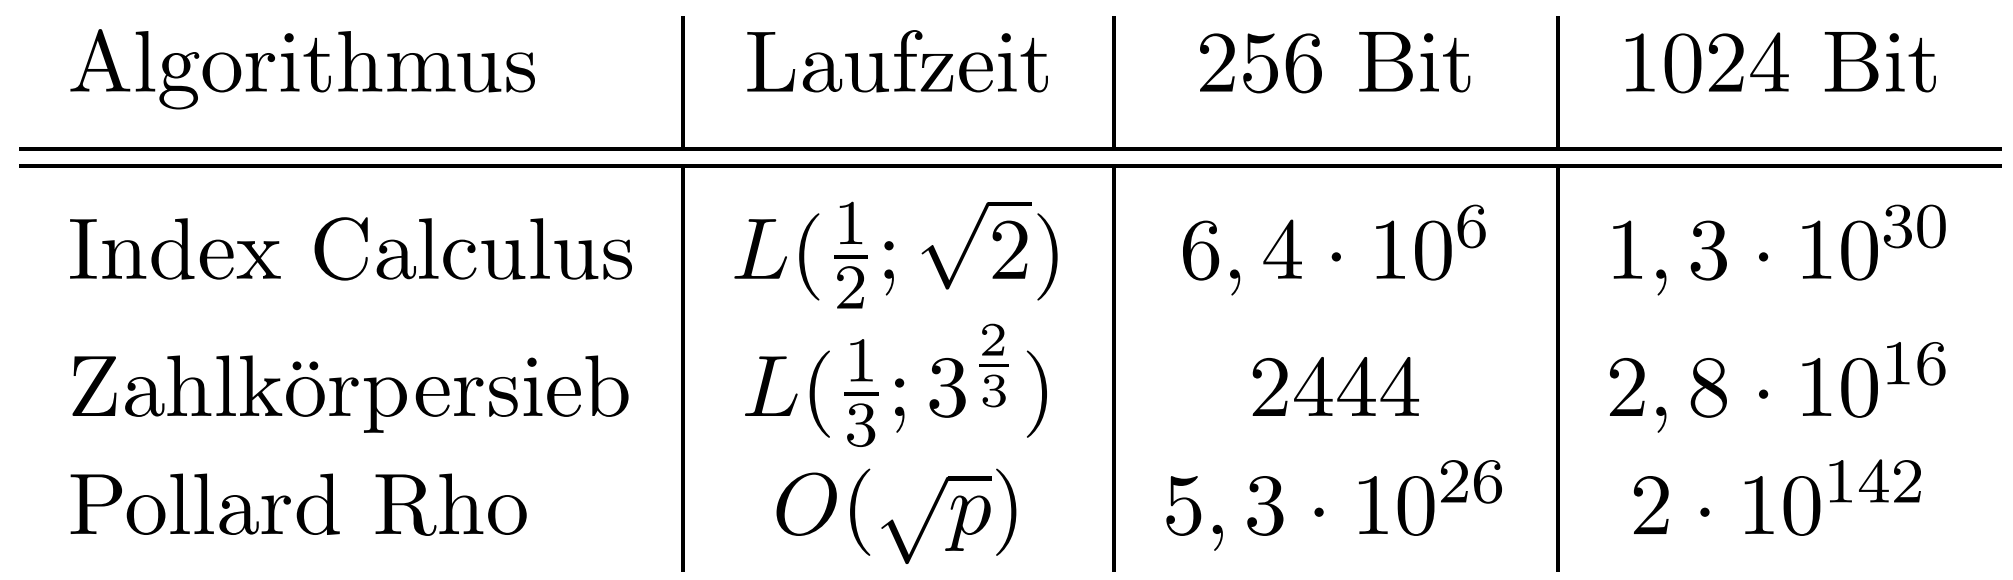
\includegraphics[width=0.4\textwidth]{includes/images/LaufzeitenDLP.PNG}
		\caption{Laufzeiten von Algorithmen für DLP~\cite{DLP:ECDLP:Probleme:und:Loesungen}}
		\label{fig_LaufzeitenDLP}
	\end{figure}
	
	\begin{figure}
		\centering
		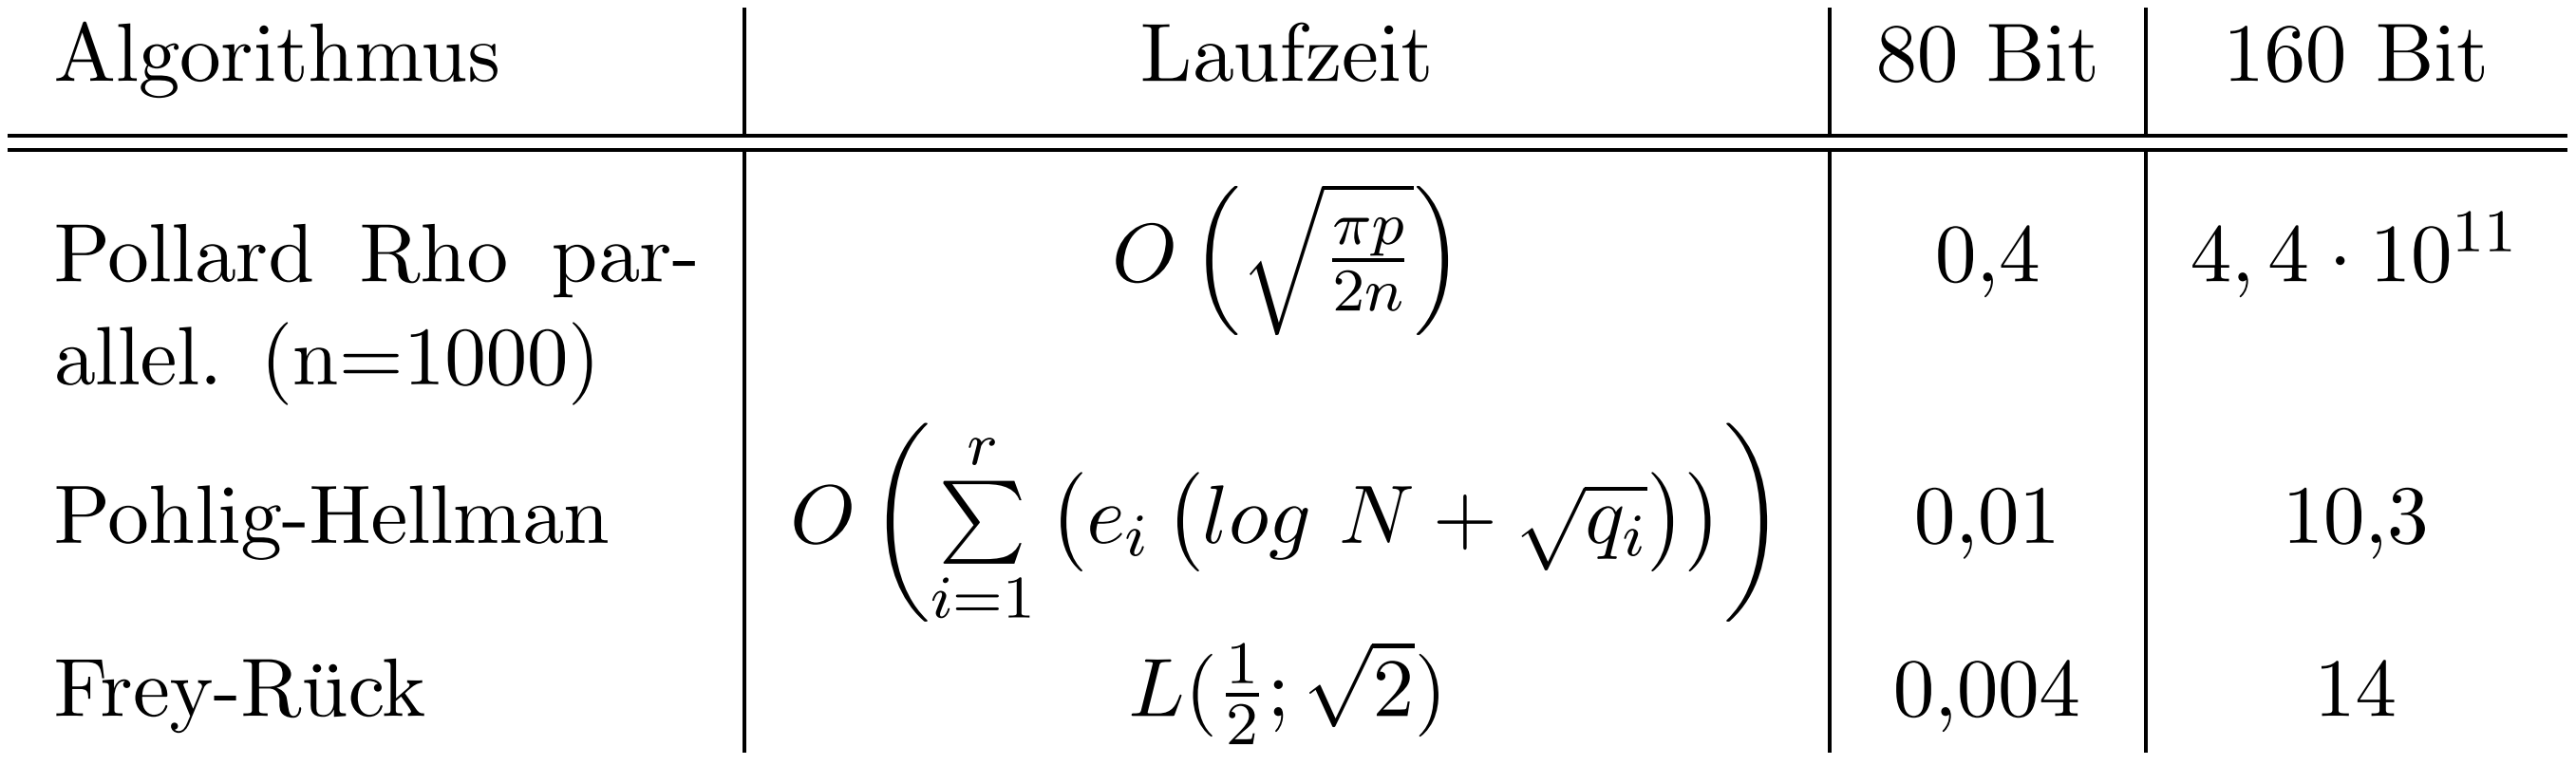
\includegraphics[width=0.5\textwidth]{includes/images/LaufzeitenECDLP.PNG}
		\caption{Laufzeiten von Algorithmen für ECDLP~\cite{DLP:ECDLP:Probleme:und:Loesungen}}
		\label{fig_LaufzeitenECDLP}
	\end{figure}
	
	Der Höhepunkt im Bereich der Verschlüsselung kann noch nicht erreicht sein. Noch schnellere und effizientere und somit \myAnfuehrungszeichen{sicherere} Verschlüsselungstechniken werden benötigt um auch zukünftigen Anforderungen gerecht zu werden. Denn die nötigen Algorithmen um sämtliche heutigen Verschlüsselungen zu brechen existieren schon, laut Peter W. Shor. Diese stellt er in \cite{Algorithms:for:Quantum:Computation:Discrete:Logarithms:and:Factoring} vor. Diskrete Logarithmen können in polynomialer Zeit berechnet werden, es muss nur noch gelingen einen Quantencomputer zu bauen.